%----------------------------------------------------------------------------------------
%   PACKAGES AND OTHER DOCUMENT CONFIGURATIONS
%----------------------------------------------------------------------------------------

\documentclass[
10pt, % Main document font size
a4paper, % Paper type, use 'letterpaper' for US Letter paper
oneside, % One page layout (no page indentation)
%twoside, % Two page layout (page indentation for binding and different headers)
headinclude,footinclude, % Extra spacing for the header and footer
BCOR5mm, % Binding correction
]{scrartcl}

\usepackage[utf8]{inputenc}
\usepackage[english]{babel}

\usepackage{geometry}
\geometry{textheight = 22cm}

\usepackage{comment}

\usepackage{graphics,graphicx}
\graphicspath{ {./figures/} }
\usepackage{amsmath}

%%%%%%%%%%%%%%%%%%%%%%%%%%%%%%%%%%%%%%%%%
% Arsclassica Article
% Structure Specification File
%
% This file has been downloaded from:
% http://www.LaTeXTemplates.com
%
% Original author:
% Lorenzo Pantieri (http://www.lorenzopantieri.net) with extensive modifications by:
% Vel (vel@latextemplates.com)
%
% License:
% CC BY-NC-SA 3.0 (http://creativecommons.org/licenses/by-nc-sa/3.0/)
%
%%%%%%%%%%%%%%%%%%%%%%%%%%%%%%%%%%%%%%%%%

%----------------------------------------------------------------------------------------
%   REQUIRED PACKAGES
%----------------------------------------------------------------------------------------

\usepackage[
nochapters, % Turn off chapters since this is an article        
beramono, % Use the Bera Mono font for monospaced text (\texttt)
eulermath,% Use the Euler font for mathematics
pdfspacing, % Makes use of pdftex’ letter spacing capabilities via the microtype package
dottedtoc % Dotted lines leading to the page numbers in the table of contents
]{classicthesis} % The layout is based on the Classic Thesis style

\usepackage{arsclassica} % Modifies the Classic Thesis package

\usepackage[T1]{fontenc} % Use 8-bit encoding that has 256 glyphs

\usepackage[utf8]{inputenc} % Required for including letters with accents

\usepackage{graphicx} % Required for including images
\graphicspath{{Figures/}} % Set the default folder for images

\usepackage{enumitem} % Required for manipulating the whitespace between and within lists

\usepackage{lipsum} % Used for inserting dummy 'Lorem ipsum' text into the template

\usepackage{subfig} % Required for creating figures with multiple parts (subfigures)

\usepackage{amsmath,amssymb,amsthm} % For including math equations, theorems, symbols, etc

\usepackage{varioref} % More descriptive referencing

%----------------------------------------------------------------------------------------
%   THEOREM STYLES
%---------------------------------------------------------------------------------------

\theoremstyle{definition} % Define theorem styles here based on the definition style (used for definitions and examples)
\newtheorem{definition}{Definition}

\theoremstyle{plain} % Define theorem styles here based on the plain style (used for theorems, lemmas, propositions)
\newtheorem{theorem}{Theorem}

\theoremstyle{remark} % Define theorem styles here based on the remark style (used for remarks and notes)

%----------------------------------------------------------------------------------------
%   HYPERLINKS
%---------------------------------------------------------------------------------------

\hypersetup{
%draft, % Uncomment to remove all links (useful for printing in black and white)
colorlinks=true, breaklinks=true, bookmarks=true,bookmarksnumbered,
urlcolor=webbrown, linkcolor=RoyalBlue, citecolor=webgreen, % Link colors
pdftitle={}, % PDF title
pdfauthor={\textcopyright}, % PDF Author
pdfsubject={}, % PDF Subject
pdfkeywords={}, % PDF Keywords
pdfcreator={pdfLaTeX}, % PDF Creator
pdfproducer={LaTeX with hyperref and ClassicThesis} % PDF producer
} % Include the structure.tex file which specified the document structure and layout

%----------------------------------------------------------------------------------------
%   TITLE AND AUTHOR(S)
%----------------------------------------------------------------------------------------

\title{\normalfont\spacedallcaps{NOtes on Magnetic field design on PROCURE}} % The article title

%\subtitle{Subtitle} % Uncomment to display a subtitle

\author{\spacedlowsmallcaps{Bruno Ximenez} }% The article author(s) - author affiliations need to be specified in the AUTHOR AFFILIATIONS block

\date{31/01/2021} % An optional date to appear under the author(s)

\begin{document}
%----------------------------------------------------------------------------------------

%----------------------------------------------------------------------------------------
%   HEADERS
%----------------------------------------------------------------------------------------

\renewcommand{\sectionmark}[1]{\markright{\spacedlowsmallcaps{#1}}} % The header for all pages (oneside) or for even pages (twoside)
%\renewcommand{\subsectionmark}[1]{\markright{\thesubsection~#1}} % Uncomment when using the twoside option - this modifies the header on odd pages
\lehead{\mbox{\llap{\small\thepage\kern1em\color{halfgray} \vline}\color{halfgray}\hspace{0.5em}\rightmark\hfil}} % The header style

\pagestyle{scrheadings} % Enable the headers specified in this block


%----------------------------------------------------------------------------------------
%   TABLE OF CONTENTS & LISTS OF FIGURES AND TABLES
%----------------------------------------------------------------------------------------

\maketitle % Print the title/author/date block

\setcounter{tocdepth}{2} % Set the depth of the table of contents to show sections and subsections only

\tableofcontents % Print the table of contents

\listoffigures % Print the list of figures

\listoftables % Print the list of tables

\newpage

\section{$\vec{B}$ field configuration study}

Here is an initial investigation on the magnetic field produced by the under-vacuum coils designed for the PROCURE machine.
The setup is a pair of solenoids with about 5 turns. I consider here as an example, solenoids with radius of 40 mm and a distance between the two solenoids (in a Helmholtz configuration) of about 80 mm or the diameter of the coils. The current chosen to plot the graphs is 20 A. On figure \ref{helmholtz}. This setup generates a highly homogeneous magnetic field at the trapping site, which has a cubic volume with a length of  l = 30 $\times$ 5 $\mu$m $\approx$ 0.15 mm.



\begin{figure}[t]
    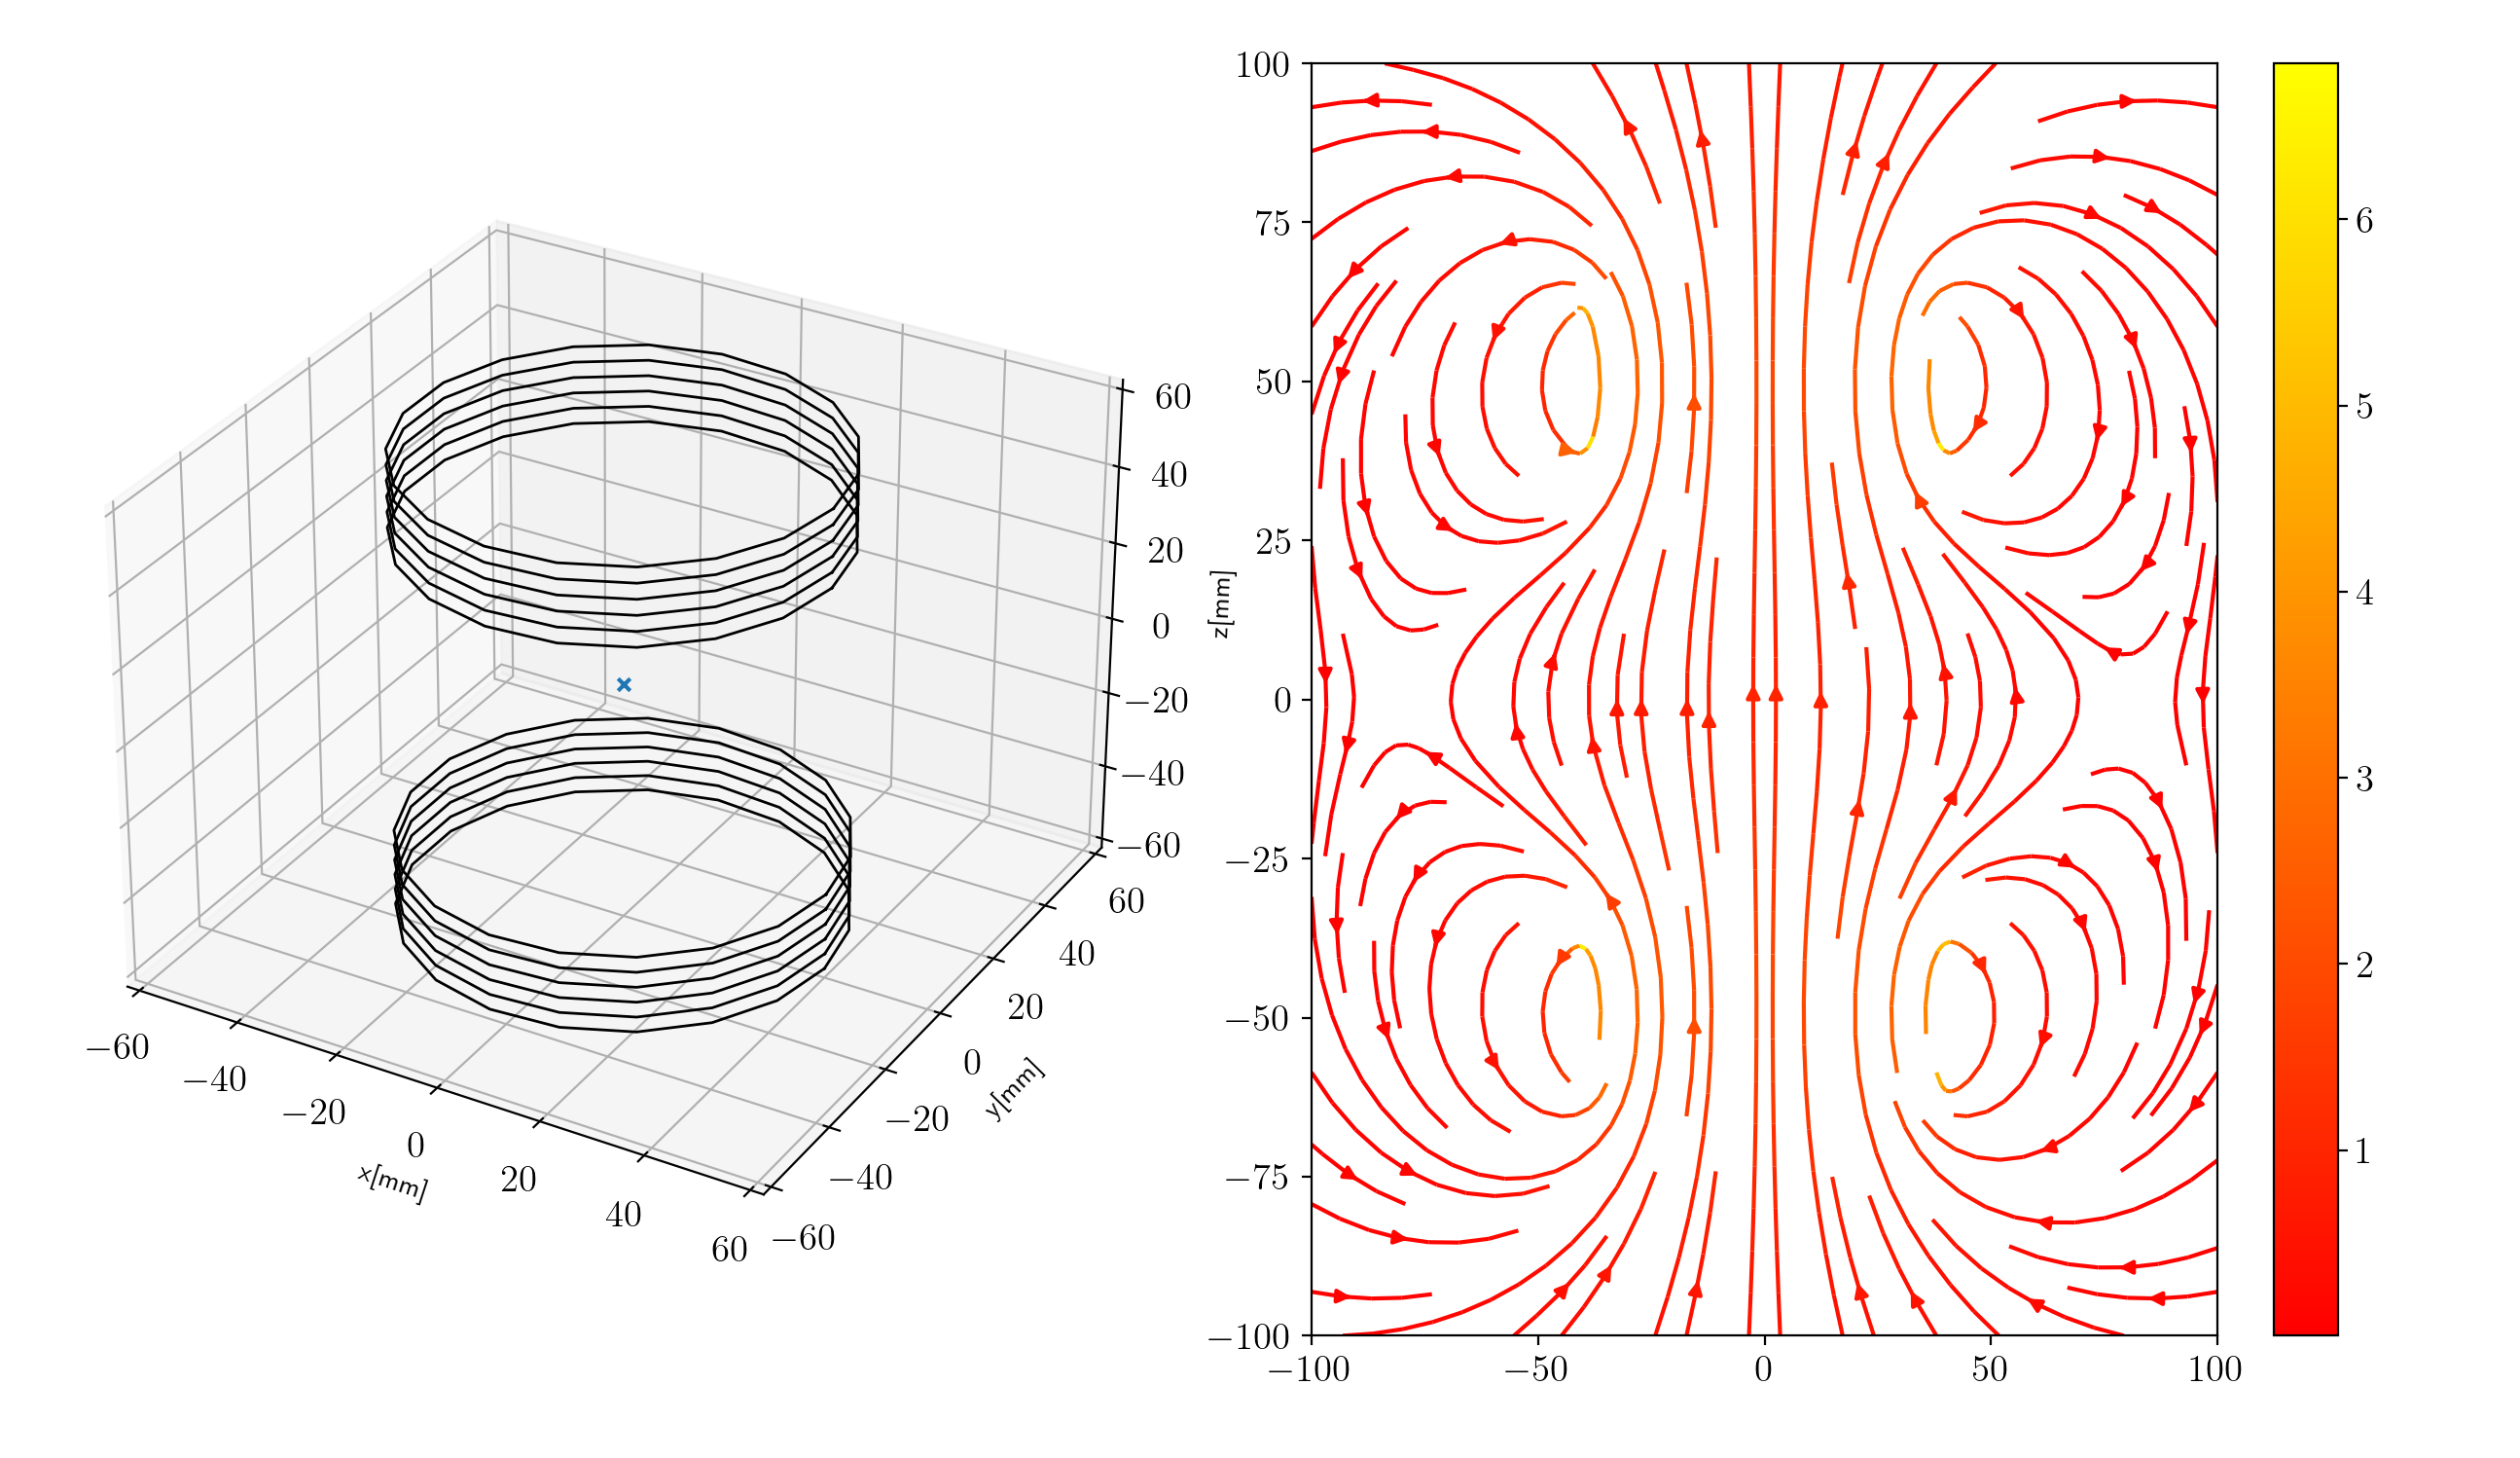
\includegraphics[width=\linewidth]{XZplane_6turns_20amps_radius40mm_d80}
    \centering
    \caption{The Helmholtz coils setup is representes on the left and on the right the line fields of the magnetic field on the XZ plane.}
    \label{helmholtz}
\end{figure}


For those parameters the magnetic field produced at the trap is on the order of 1 mT. Varying the distance between the coils by 2 mm leads to a change on the magnitude of the field on the order of $10^{-2}$ mT but the homegeneity is kept nearly the same, which is on the order of $\mu$T. Results are shown on figure \ref{dist}.


\begin{figure}[t]
    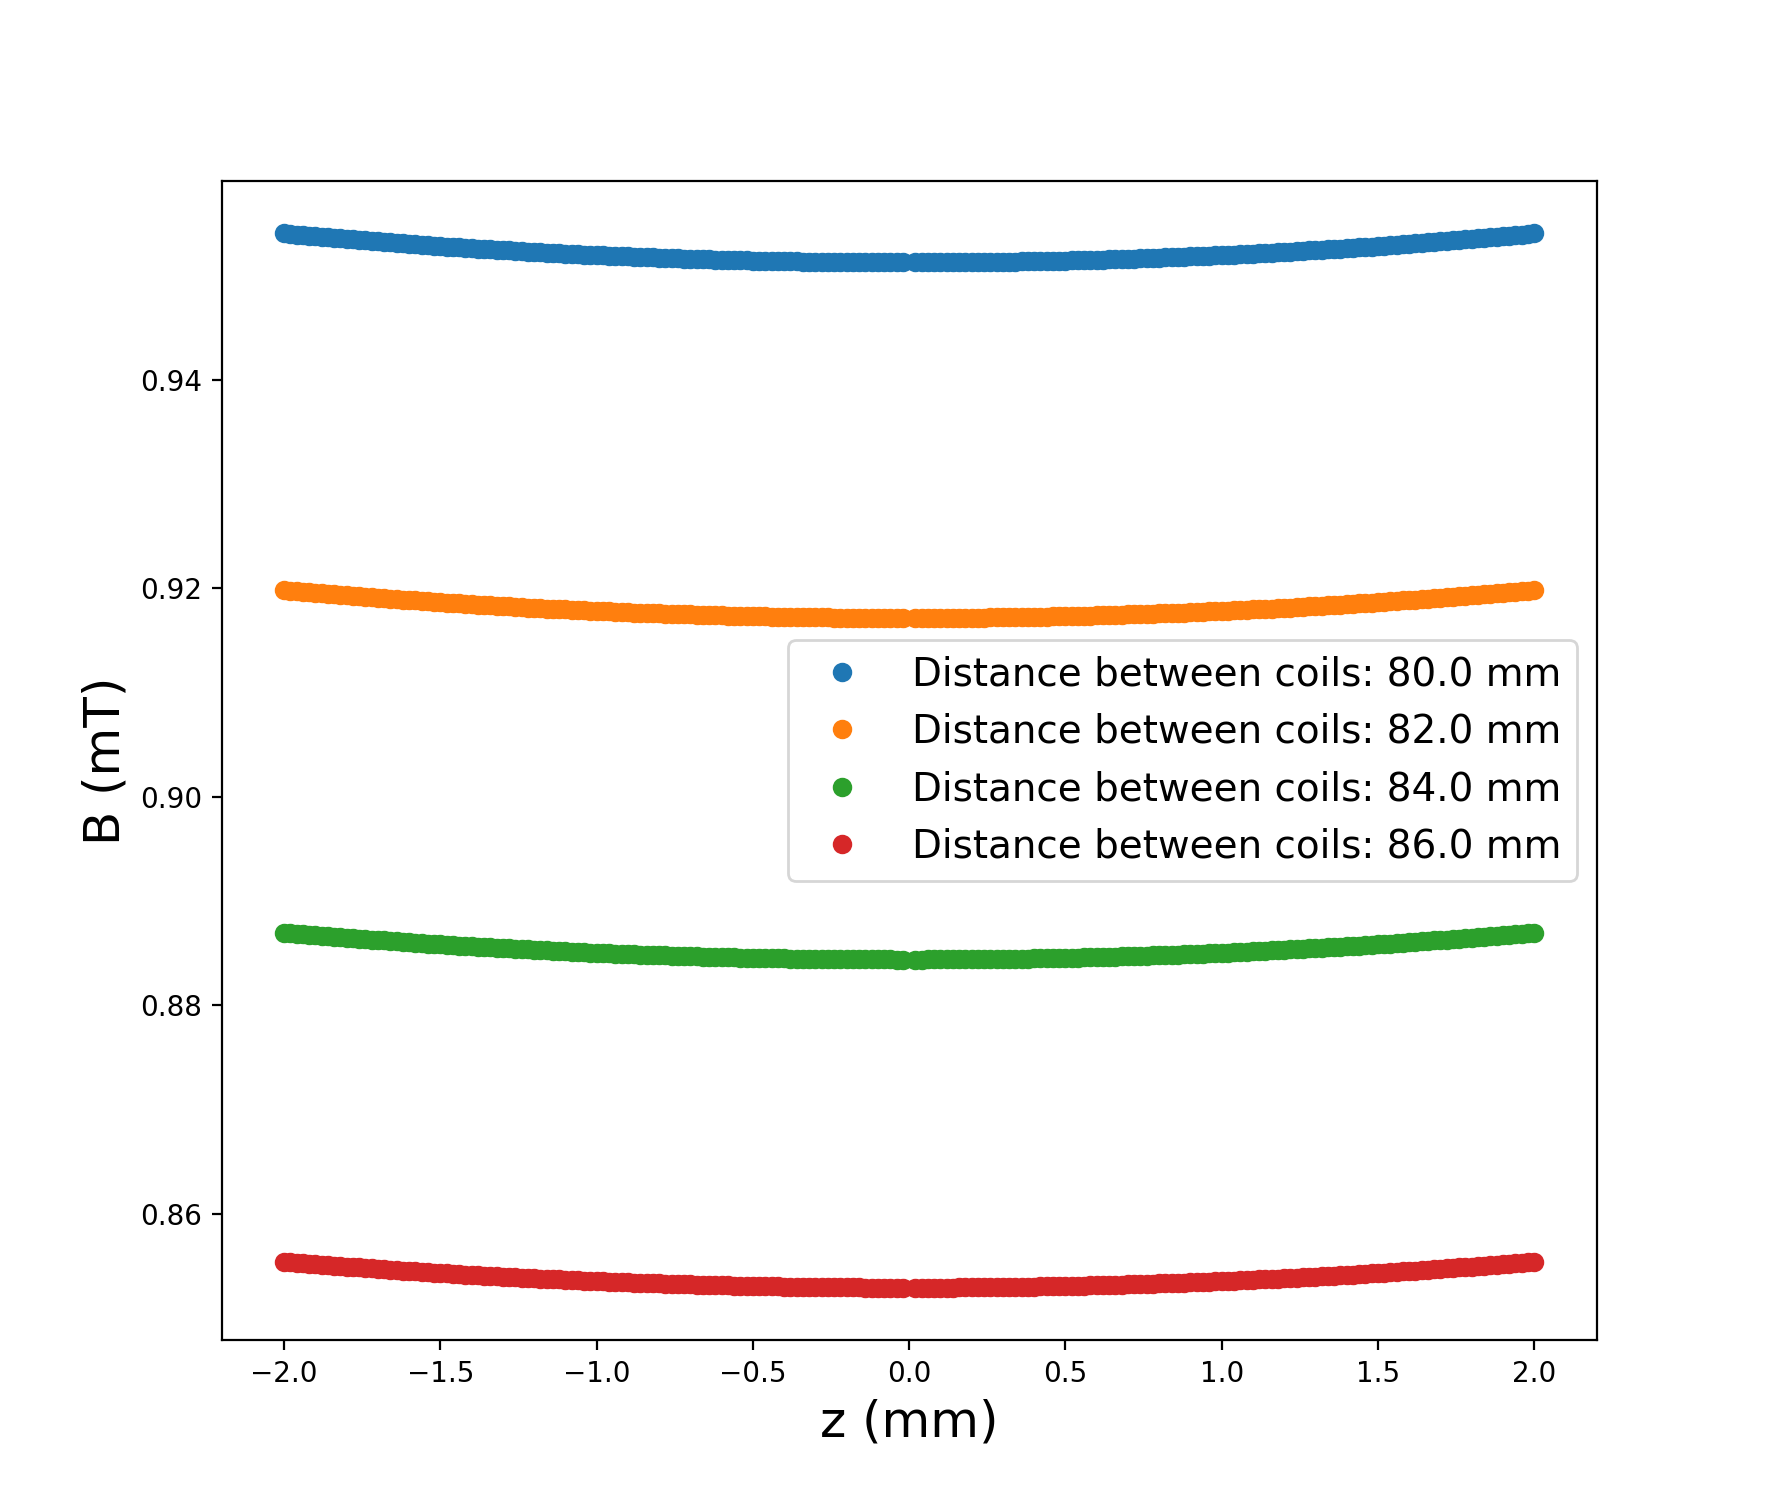
\includegraphics[width=\linewidth]{varying_distance_between_coils.png}
    \centering
    \caption{Magnitude of the magnetic field produced on the z-axis when varying the distance between the coils.}
    \label{dist}
\end{figure}

Next I tilt the one of the coils by about 10 degrees. On figure \ref{tilted_coil} is shown the geometric deformation and on figure \ref{tilted_coil_B} is the magnitude of the magnetic field on the z-axis. There is a shift on the minimum of the magnetic field and variations on the magnetic field on the level of $10^{-3}$ mT.

\begin{figure}[t]
    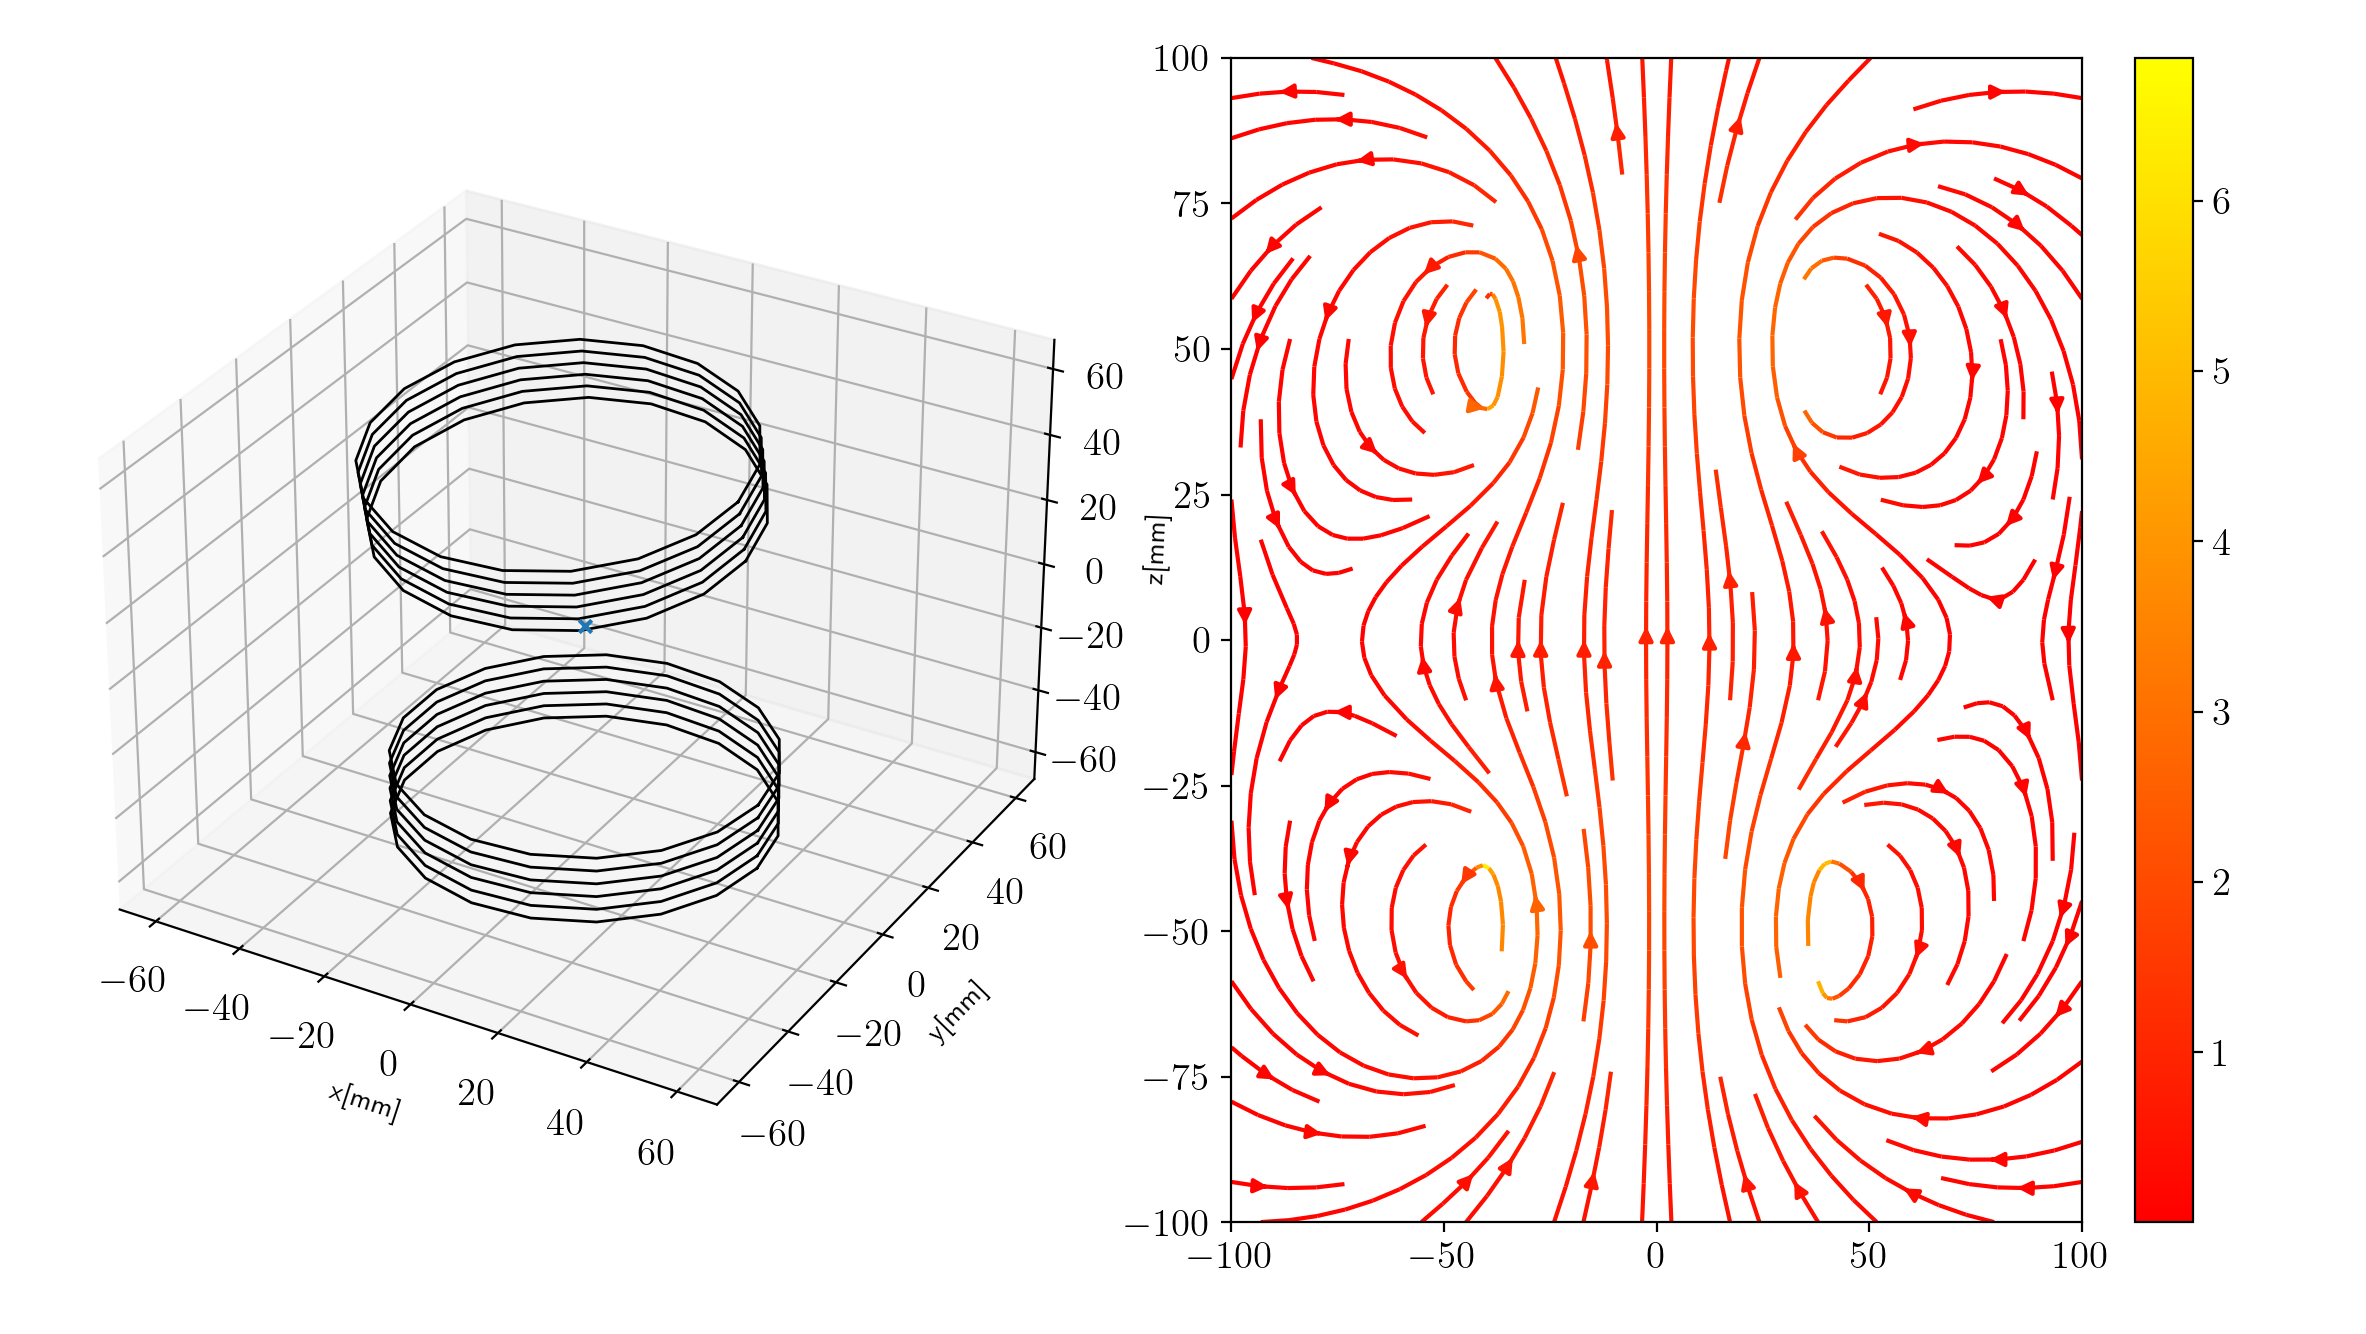
\includegraphics[width=\linewidth]{Tilted_coil_10Deg}
    \centering
    \caption{Tilted coil of 10 degrees.}
    \label{tilted_coil}
\end{figure}

\begin{figure}[t]
    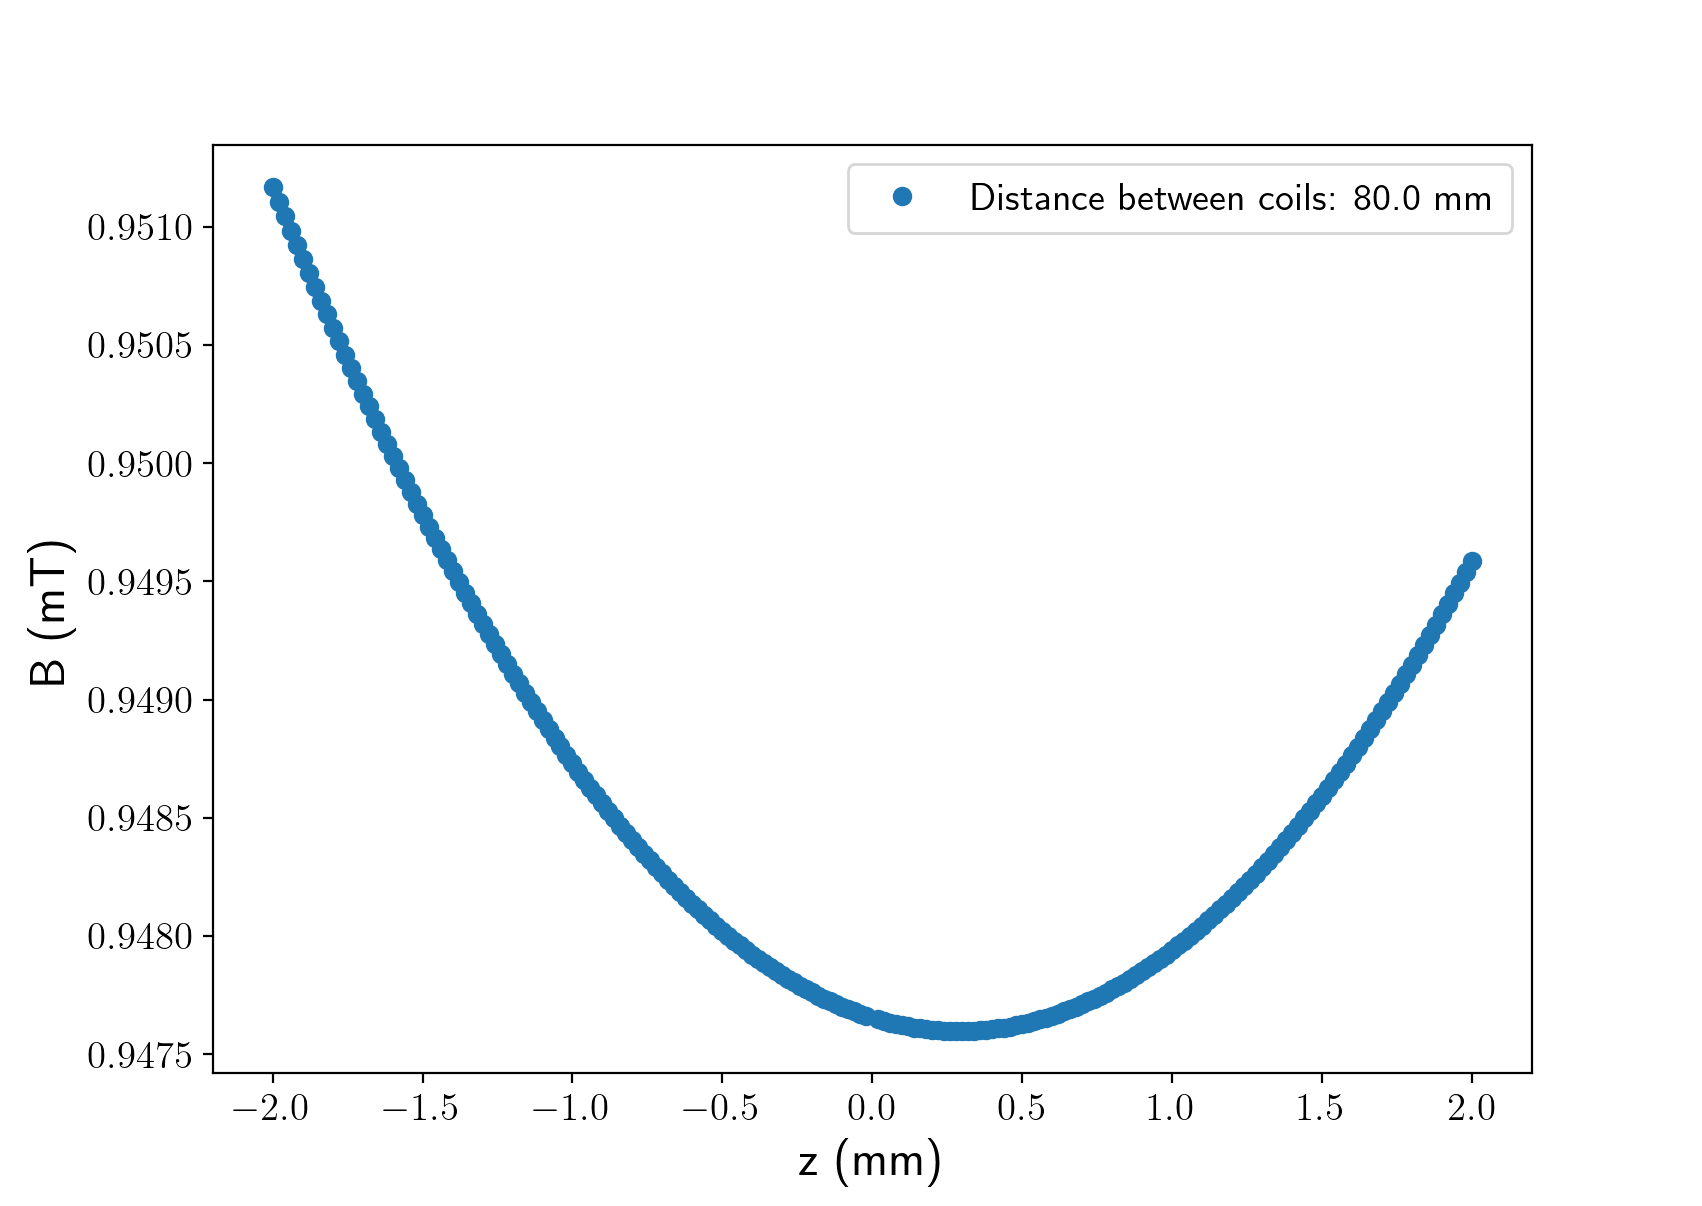
\includegraphics[width=\linewidth]{TiltedCoil10Deg_B}
    \centering
    \caption{Tilted coil of 10 degrees.}
    \label{tilted_coil_B}
\end{figure}

We can conclude that we don't need to worry too much about the exact geometry of the solenoid for homogenous magnetic field at the level of $\mu$T (or better than 0.1 Gauss), in this approximation and in the trapping region of about 0.15 mm. 

\newpage

\section{Heat dissipated on the coils}

Considering ideal coils with N turns copper wire with a given diameter, the resistance of the solenoid is given by:

\begin{equation}
    R_{solenoid} = \frac{L\rho}{\pi r_{wire}^{2}},
\end{equation}
where $\rho$ is the resistance of the copper, L is the length of the wire making the solenoid and $r_{wire}$ is the radius of the wire. The length of the wire can be approximated as $L = 2\pi \rho_{solenoid} N$, being $rho_{solenoid}$ the radius of each turn.

The total resistance of the solenoid is:

\begin{equation}
    R_{solenoid} = \frac{2 \rho_{solenoid} N \rho_{copper} I^{2}}{r_{wire}^{2}}
\end{equation}

The power dissipated is just $RI^{2}$ and as a scaling law:

\begin{equation}
    P \approx N (I / r_{wire})^{2}
\end{equation}

If we want to dissipate as minimum heat as we can, thicker wire and maximize the number of turns in the solenoid is desired. If the number of turn in the solenoid is increased by a factor of f then the dissipated power is reduced by a fact of f. Considering a 1.5 mm radius wire and $\rho_{copper} = 0.0171$ $\Omega$ mm $^{2}$/m, and a solenoid with 4 turns, that gives a total lentgh of about 1 m, a total resistance of about 2 m$\Omega$ and $I = 20$ A, then 1 W will be dissipated as heat on each solenoid.


\section{Zeeman effect on $^{87}$Rb}

\end{document}